\RequirePackage{plautopatch}

\documentclass[a4paper, 11pt]{ltjsarticle}


% マージン設定
\usepackage[top=20mm, bottom=20mm, left=20mm, right=20mm]{geometry}

% LuaLaTeX用日本語対応パッケージ
\usepackage{luatexja}
\usepackage{luatexja-fontspec}

% 必要なパッケージ
\usepackage{fontspec}
\usepackage{titlesec}
\usepackage{graphicx}
\usepackage{amsmath}
\usepackage{amssymb}
\usepackage[colorlinks=true, linkcolor=black, citecolor=black]{hyperref}
\usepackage{tocloft}
\usepackage{indentfirst}
\usepackage{tikz} % カスタム点線用
\usepackage{here}
\usepackage{caption}
\usepackage{bookmark}
\usepackage{multicol}
\usepackage{multirow}
\usepackage{flushend}
\usepackage{subfig}
\usepackage{threeparttable}
\usepackage{enumitem}
\usepackage{url}
\usepackage{svg}

% 図:1のコロンを消す
\captionsetup{labelsep=space}

% 参考文献を上付きにする
\usepackage[super]{cite}
\renewcommand\citeform[1]{[#1]}

\setlength{\baselineskip}{14pt}
\setlength{\parindent}{1\zw}

\titleformat{\section}{\large\bfseries}{\thesection.}{1\zw}{}
\titleformat{\subsection}{\large\bfseries}{\thesubsection.}{1\zw}{}
\titleformat{\subsubsection}{\large\bfseries}{\thesubsubsection.}{1\zw}{}

\setcounter{tocdepth}{3}
\makeatletter
\renewcommand{\numberline}[1]{#1.~}
\renewcommand{\cftsecleader}{\cftdotfill{\cftdotsep}}
\renewcommand{\cftsubsecleader}{\hfill}
\renewcommand{\cftsubsubsecleader}{\hfill}
\cftpagenumbersoff{subsection}
\cftpagenumbersoff{subsubsection}
\makeatother

\DeclareCaptionFont{designatedFont}{\fontsize{11pt}{14pt}\selectfont}
\captionsetup{font=designatedFont}

%---ここから中身---------------------------------------------------------------------------------------
\begin{document}
\fontsize{11pt}{14pt}\selectfont

%---表紙---------------------------------------------------------------------------------------
\thispagestyle{empty}
\begin{center}
\pagenumbering{gobble}  %ページ番号をカウントしない

\vspace*{40mm}
{\huge\noindent 災害時を想定したアドホックネットワーク}\\
\medskip
{\huge\noindent 構築手法の検討}\\
\vspace{\baselineskip}
{\huge\noindent\textbf{Study of Construction Methods for Ad-Hoc Network under Disaster}}\\
\vspace{120mm}

{\huge\noindent
2025年3月4日\\
東京都立産業技術高等専門学校\\
ものづくり工学科 情報通信工学コース \\
末廣 隼人\\
指導教員 髙﨑 和之    \\
}
\vspace{40mm}

\end{center}

%---目次------------------------------------------------------------------------------------------
\clearpage  %新しいページの追加
\thispagestyle{empty}
\tableofcontents  %目次の自動生成 目次をクリックするとその章,節に飛ぶことができる

%---はじめに---------------------------------------------------------------------------------------
\clearpage
\pagenumbering{arabic}
\section{はじめに}

% ・日本では地震をはじめ多くの自然災害が発生しており,災害時には通信ネットワークが使えなくなる可能性がある.
% そこで,アドホックネットワークを活用し地域限定ながら被災状況の把握や情報伝達を可能とする研究が行われている.\\
% ・本研究では,人口密度に応じた経路構築方法を考案し,その効果をシミュレーションを用いて検証した.\\
% ・近年,Bluetoothの開発が活発に行われており,従来のBluetooth Basic Rate/Enhanced Data Rate(BR/EDR)と比べて
% 大幅な省電力化が行われたBluetooth Low Energy(BLE)が発表された.そして,\\
% ・地震などの大きな災害が発生した際,従来の基地局を用いたネットワークへのアクセスの集中等により使用できなくなった場合,
% 新たなコミュニケーション環境の実現手段として,アドホックネットワークの研究が行われている.



%---理論---------------------------------------------------------------------------------------
\clearpage
\section{理論}
\subsection{アドホックネットワークについて}
アドホックネットワークとは,中央の管理者やルータ,アクセスポイントなどの既存のインフラストラクチャを介さずに,
端末(以下では,ノードと呼ぶ)同士が直接通信を行う一時的なネットワークのことである.
電波が届かず直接情報を交換できないノード同士の場合,基地局を経由せずに途中のノードが中継するマルチホップ通信により情報交換が可能になる.
これらを踏まえると,ノードさえあればどのようなエリアでも即席にネットワークを形成することができるためとても便利だが,
ノード移動に伴うネットワークトポロジや伝送品質の急激な変化,利用可能な無線周波数帯域の限界,バッテリ依存のノードの消費電力などの制約といった
厳しい条件がある.そのため,ルーティングやチャネルアクセスの制御,周波数帯域の有効活用,ノードの電力消費の節約等の多くの課題がある\cite{間瀬憲一2001アドホックネットワーク}.

アドホックネットワークに関する研究の歴史は長く,第1世代であるアドホックネットワーク"PRNET(Packet Radio Network)"
は1972年に米国の国防高等研究計画局によって開発され,軍事利用を目的とした研究のため実用化には至らなかった.
次に,第2世代となる"NTDR(Near-term Digital Radio)"も米国により軍事目的で研究が行われ,1980年代頃から実用化されている.
そして,第3世代となる"MANET(Mobile Ad hoc NETwork)"を含む現在のアドホックネットワーク技術はIEEE802.11やBluetoothなどの
近距離無線通信技術を活用し,民間でも使用できるアドホックネットワークが2000年頃から誕生した.同時期から災害時用ネットワークとして
の活用に期待が高まっていた.\\

図1のように無線マルチホップを利用したアドホックネットワークのイメージ図である.

% \indent アドホックネットワークに関する研究の歴史が長く,1970年代初頭に軍事利用の観点から研究が開始された.1990年代半ばから世界的に研究が活発になり,1997年にはIETF(Internet Engineering Task Force)
% にMANET(Mobile Ad hoc NETwork)WGが発足され,ルーティングプロトコルを中心とした標準化の議論も開始された.

\subsection{ルーティング方式}
ルーティングプロトコルは大きくリアクティブ型,プロアクティブ型,ハイブリッド型の3つに分類される(図\ref{routing_classification}).
次節にそれぞれの特徴と簡単な概略図を用いて紹介を行う.
\begin{figure}[H]
  \centering
  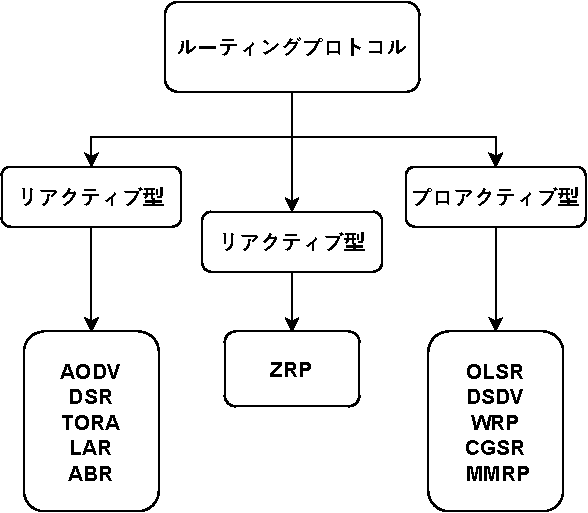
\includegraphics[width=80mm]{classification_of_routing.pdf}
  \caption{ルーティングテーブルの分類}
  \label{routing_classification}
\end{figure}

% \clearpage
\subsubsection{リアクティブ型}
\subsubsection{プロアクティブ型}
\subsubsection{ハイブリッド型}
% \subsection{アドホックネットワークの技術的課題}
% \subsubsection{隠れ端末問題}
% 隠れ端末問題とは、図1のようにノードAとCがノードBに対して通信を行うとき、ノードAとCはお互いの存在が隠れてしまい、
% 現在誰も通信を行なってないと思い込んで同時にノードBへと通信を行いデータが衝突してし壊れてしまう問題である。%
% \begin{figure}[H]
%   \centering
%   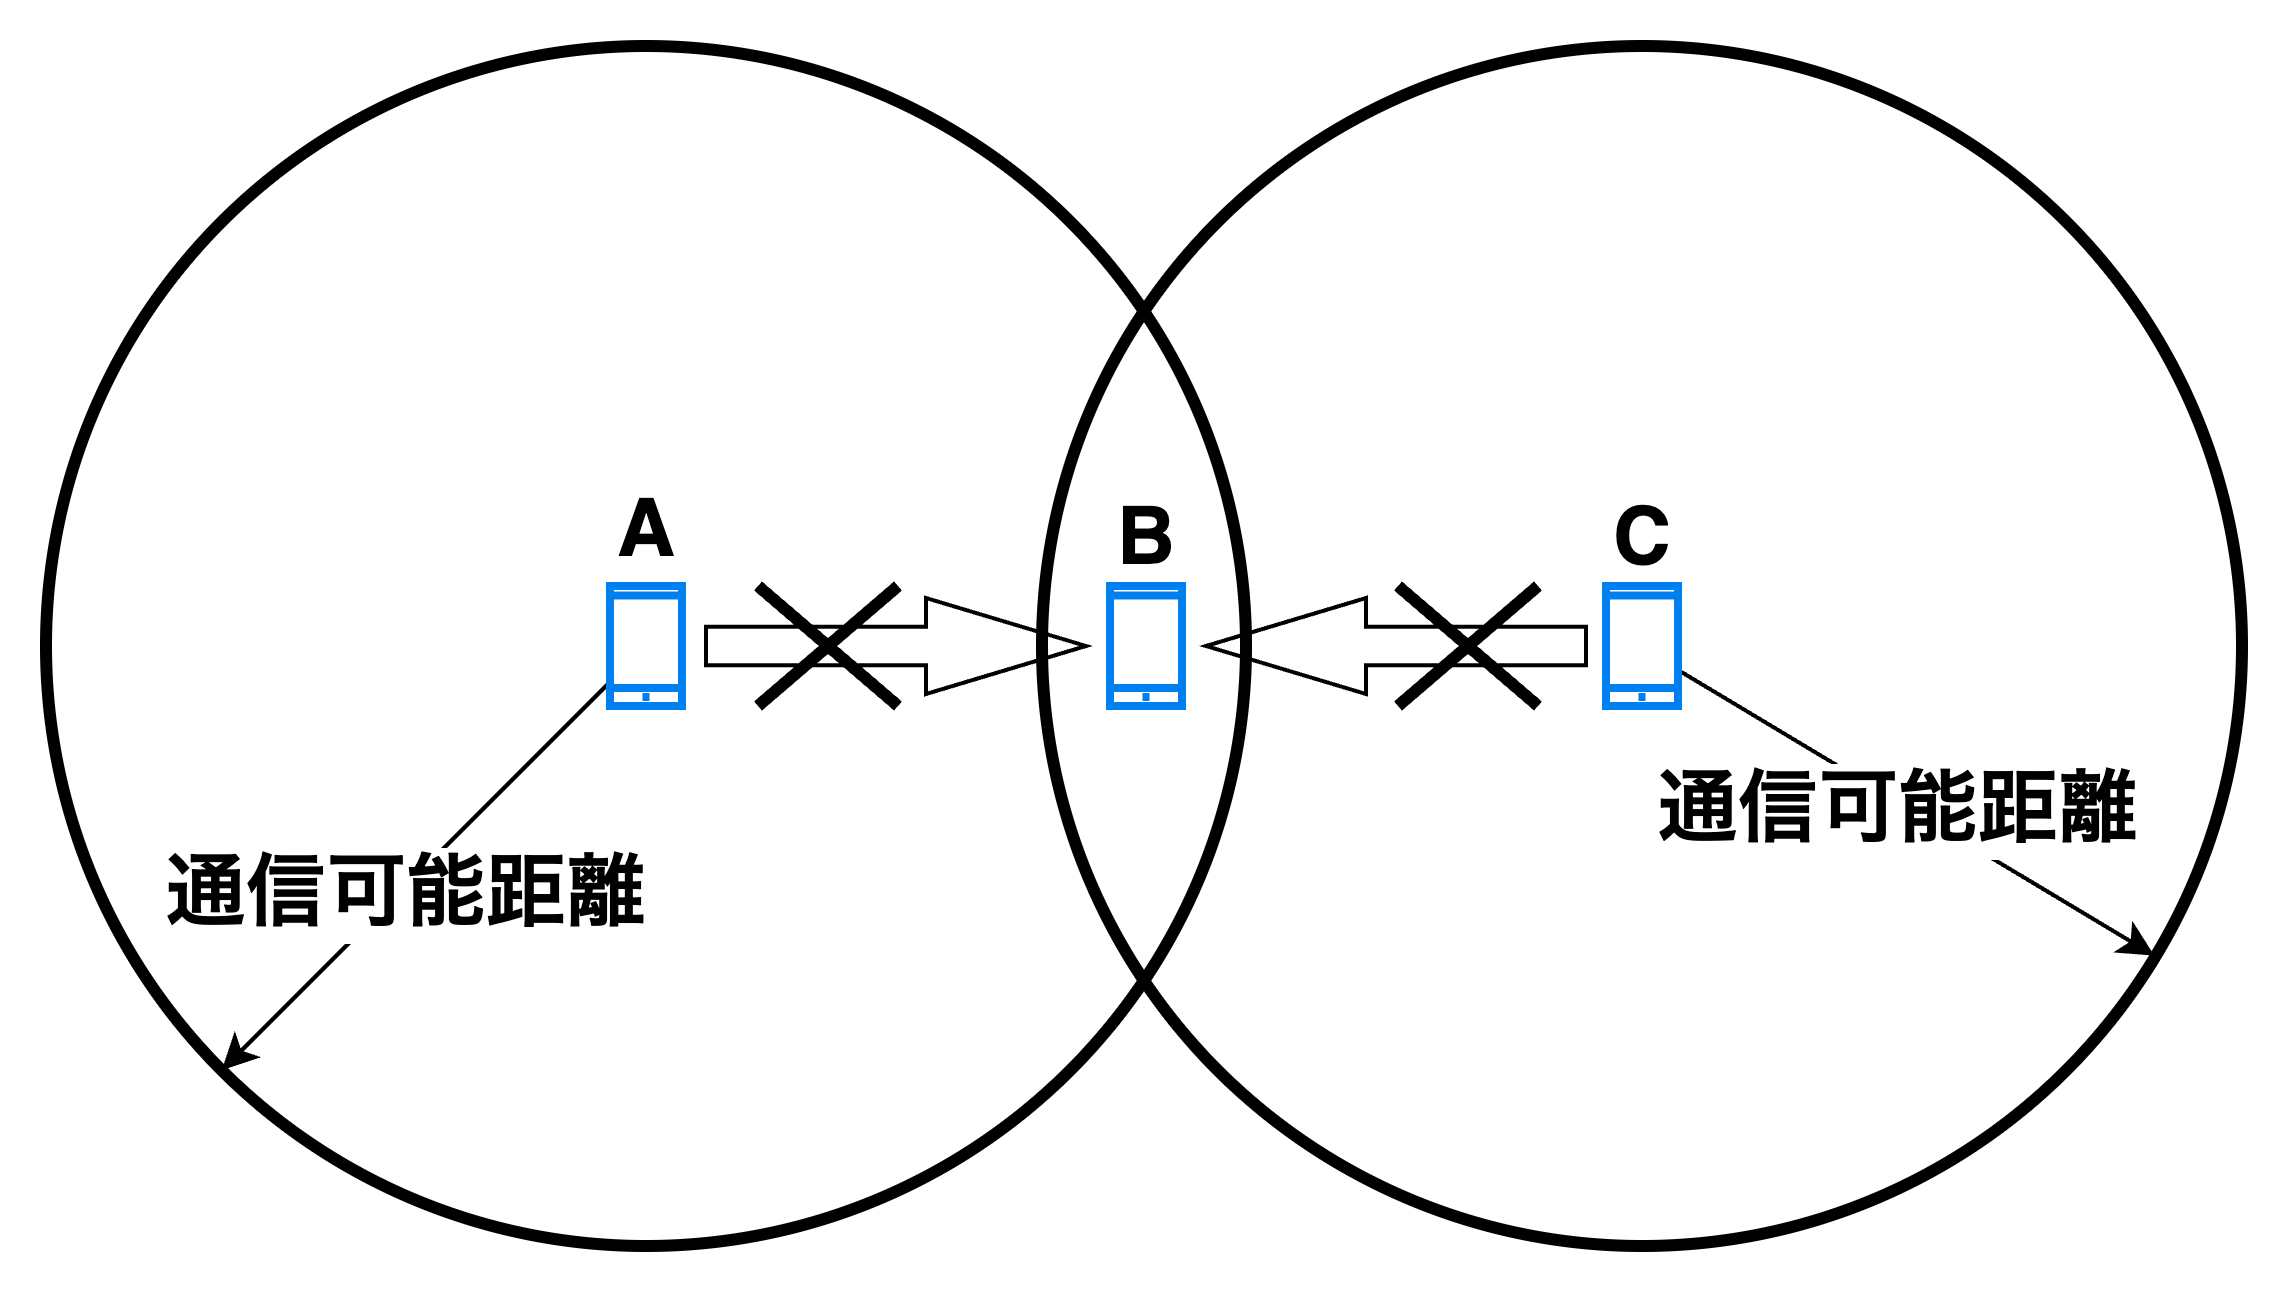
\includegraphics[width=70mm]{hidden_terminal_problem.png}
%   \caption{隠れ端末問題}
% \end{figure}

% \subsubsection{さらし端末問題}
% さらし端末問題\cite{人口密度}とは、図2のようにノードAがDと通信を行なっているときノードBは端末Cと通信ができそうだが、
% ノードAがDと通信を行なっているため周辺にいる他ノードは通信の抑制がされてしまい、
% 伝送速度や通信品質の低下が発生してしまう問題である。%
% \begin{figure}[H]
%   \centering
%   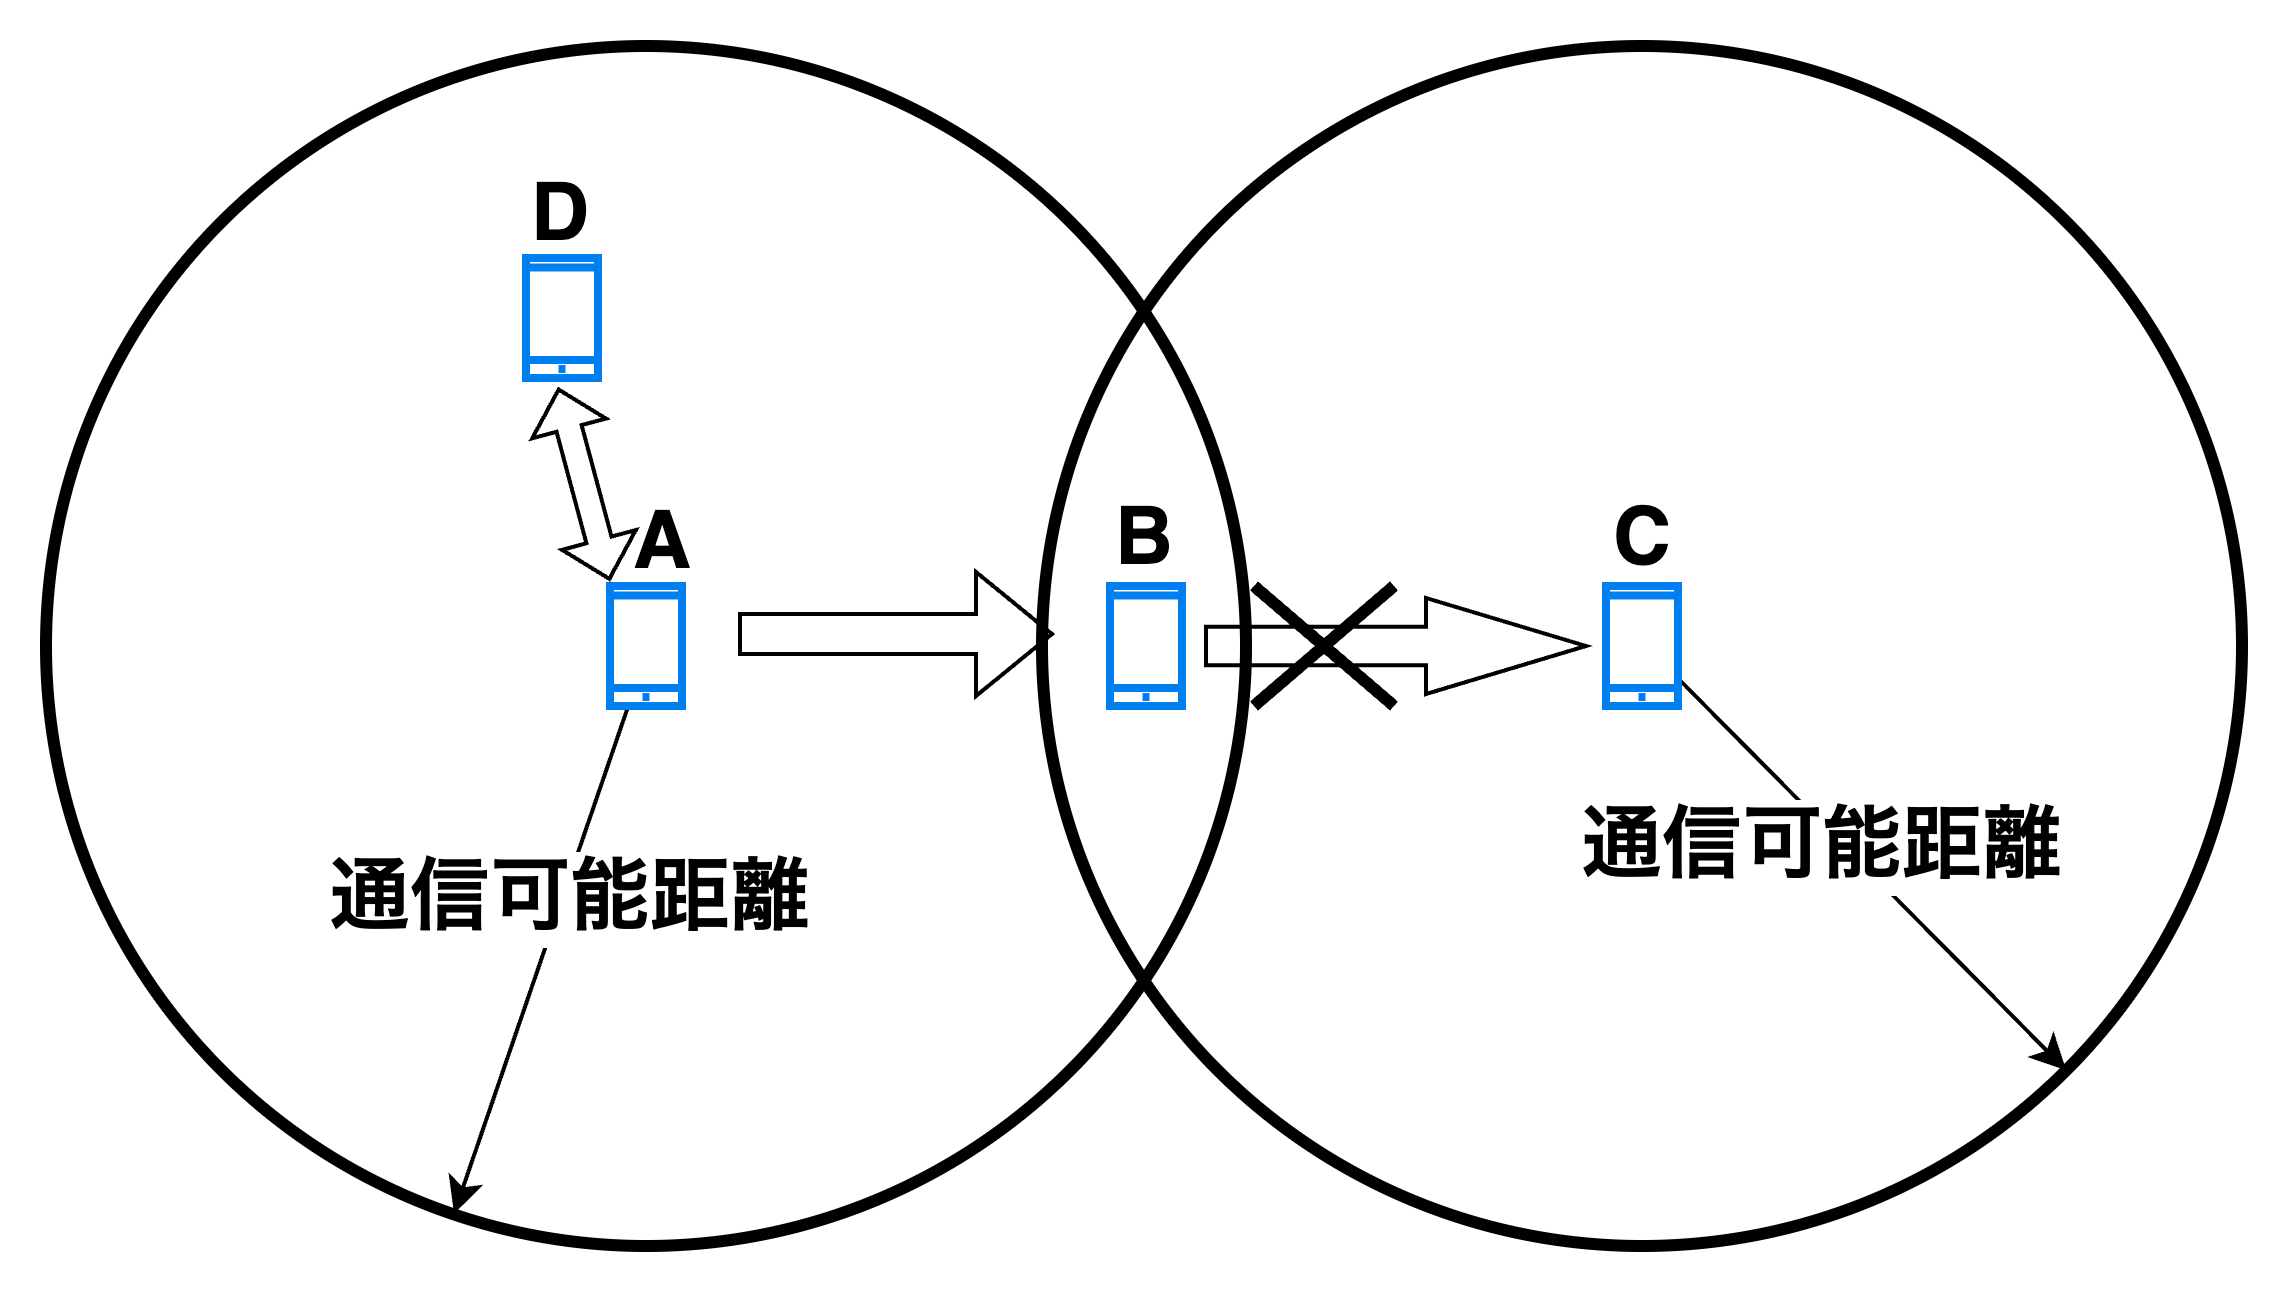
\includegraphics[width=70mm]{exposed_terminal_problem.png}
%   \caption{さらし端末問題}
% \end{figure}
\subsection{Bluetoothの規格について}

%---提案手法---------------------------------------------------------------------------------------
\clearpage
\section{提案手法}

%---結果---------------------------------------------------------------------------------------
\clearpage
\section{結果}

%---考察とまとめ---------------------------------------------------------------------------------------
\clearpage
\section{考察とまとめ}

%---参考文献---------------------------------------------------------------------------------------
\clearpage
\addcontentsline{toc}{section}{参考文献}
\bibliography{arxiv}
\bibliographystyle{junsrt}


\end{document}